\documentclass[slide,papersize]{jsarticle}
\usepackage[dvipdfmx]{graphicx,color}
\begin{document}

\section*{MapView}
\vspace*{15mm}
\begin{center}
{\Huge {\bf Google Map}}
\end{center}

\section*{やること}
\bigskip
\begin{itemize}
\item Google Maps API Key の取得
\bigskip
\item 一番簡単なサンプル
\bigskip
\item Zoom とか移動とか
\bigskip
\item 画面の回転についてフォロー
\end{itemize}

\section*{Maps API Key 取得手順}
\medskip
\begin{itemize}
\item Google アカウントの取得
\medskip
\item SDK 証明書の fingerprint 取得
\medskip
\item API Key なサイトに fingerprint 登録
\medskip
\item 登録サイト http://bit.ly/9m54x4
\medskip
\item API Key の取得
\end{itemize}

\section*{Google アカウントの取得}
\bigskip
\begin{itemize}
\item 下記より適宜アカウント取得
\bigskip
\item http://bit.ly/1vXXu4
\end{itemize}


\section*{SDK 証明書の fingerprint 取得}
\bigskip
\begin{itemize}
\item 以下に示すコマンドにて取得可能
\bigskip
\item {\scriptsize \begin{verbatim}$ keytool -list -keystore "~/.android/debug.keystore" \end{verbatim}}
\bigskip
\item debug.keystore の位置は適宜調べること
\bigskip
\item 出力される keystore をコピーしておく必要があります
\end{itemize}

\section*{fingerprint 登録}
\bigskip
\begin{itemize}
\item 前項でコピーした keystore を以下に登録
\bigskip
\item http://bit.ly/9m54x4
\end{itemize}

\section*{API Key の取得}
\bigskip
\begin{itemize}
\item 表示されるキーを保存しておきましょう
\bigskip
\item MapView オブジェクトを生成する際に必要となります
\end{itemize}

\section*{サンプルの作成 (手順)}
\bigskip
\begin{itemize}
\item Activity は MapActivity を継承
\bigskip
\item isRouteDisplayed 実装
\bigskip
\item MapView オブジェクト生成
\bigskip
\item setContentView メソドに渡す
\bigskip
\item Manifest への追記
\end{itemize}

\section*{やってみよう}
\bigskip
\begin{itemize}
\item Project Name : MapViewSample
\medskip
\item Build Target : Google APIs 1.6
\medskip
\item Application name : MapView
\medskip
\item Package name : com.example.mvs
\medskip
\item Create Activity : HelloActivity
\end{itemize}

%%\begin{verbatim}
%%{(^ ^)} (打ち込んだ通り)
%%\end{verbatim}

\section*{MapActivity の継承}
\medskip
Activity は MapActivity を継承させる
\medskip
{\scriptsize
\begin{verbatim}
public class HelloActivity extends Activity {
\end{verbatim}
}
\medskip
{\scriptsize
\begin{verbatim}
public class HelloActivity extends MapActivity {
\end{verbatim}
}

\section*{isRouteDisplayed メソドの実装}
\bigskip
\begin{itemize}
\item MapActivity を import します
\bigskip
\item Source → Override/Implement Methods 選択
\bigskip
\item isRouteDisplayed をチェックして OK
\end{itemize}

\section*{MapView オブジェクト}
%%\medskip
いっちゃん簡単なサンプルが以下。
\begin{center}
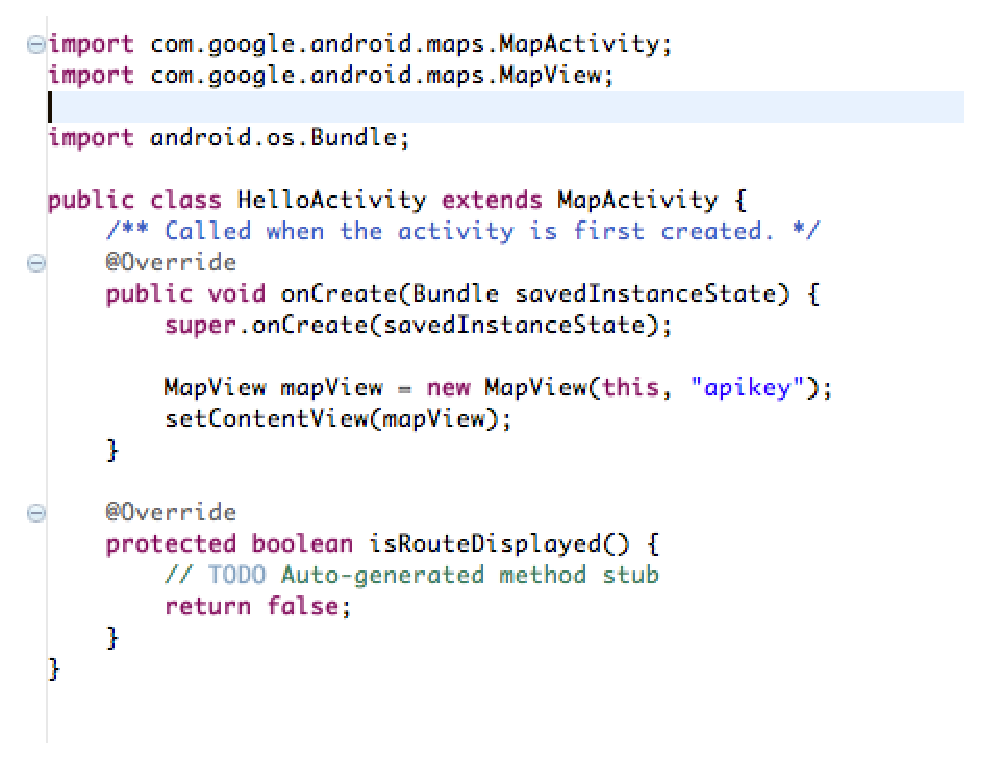
\includegraphics[scale=0.28]{MapViewSample.eps}
\end{center}

\section*{最後に Android Manifest}
%%\bigskip
使用ライブラリの追記
\begin{center}
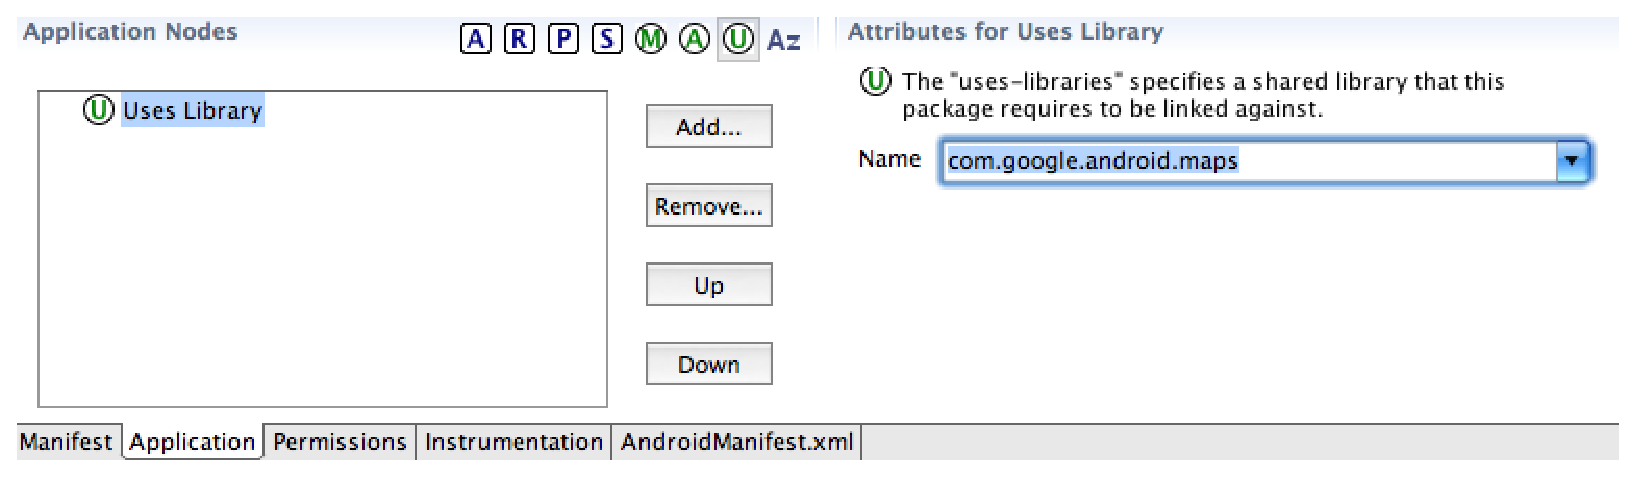
\includegraphics[scale=0.28]{uses-library.eps}
\end{center}

\section*{最後に Android Manifest}
%%\bigskip
パーミッション
\begin{center}
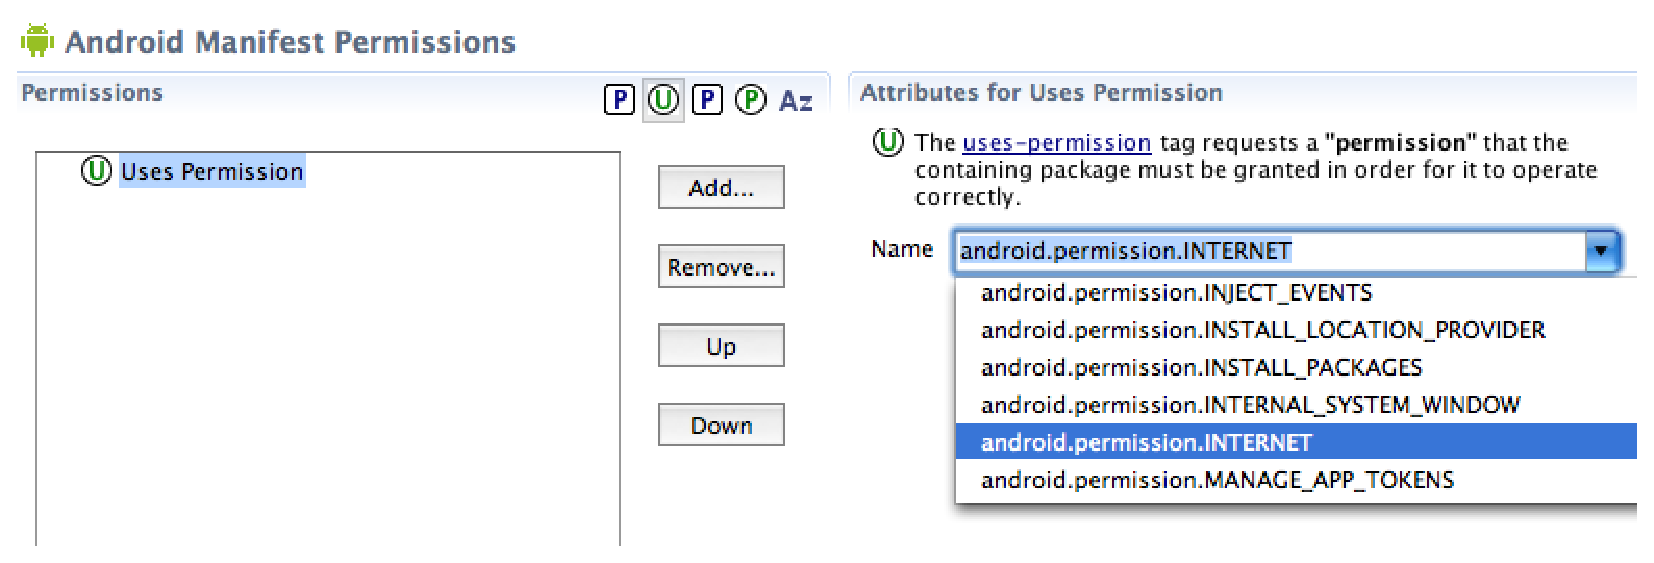
\includegraphics[scale=0.25]{internet-permission.eps}
\end{center}

\section*{できあがり}
\bigskip
\begin{itemize}
\item できあがり
\bigskip
\item 動かしてみましょう
\bigskip
\item 微妙では? (出ただけ的な意味で
\end{itemize}

\section*{Zoom とか}
\medskip
以下の二行を追加してみましょう
\begin{center}
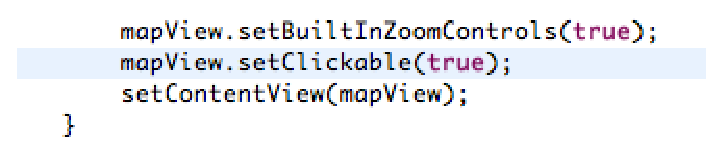
\includegraphics[scale=0.5]{clickableAndZoomable.eps}
\end{center}
Zoom できて動かせるようになります

\section*{初期表示レベル}
\bigskip
\begin{itemize}
\item 初期表示時の Zoom レベルも設定可能
\bigskip
\item MapView\#getController().setZoom(数値)
\bigskip
\item 数値を色々試してみましょう
\end{itemize}

\section*{おまけ (画面の回転)}
\bigskip
\begin{itemize}
\item 画面が回転する度に onDestroy → onCreate が呼ばれる
\bigskip
\item Log 出力確認をしてみましょう
\end{itemize}

\section*{おまけ (回転の抑制)}
\medskip
マニフェストの修正で抑制可能
\begin{center}
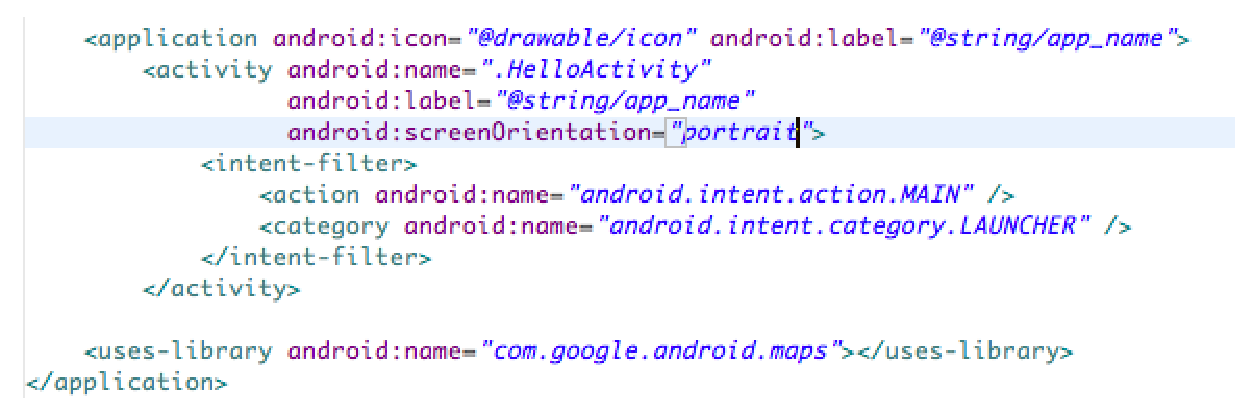
\includegraphics[scale=0.3]{portrait.eps}
\end{center}
landscape だと横専用になります

\end{document}
